\section{R�alisation}

\subsection{Transformation de mod�les}

\subsection{Les m�ta mod�les}
\begin{frame}{Diagramme de s�quence}
    \centering
    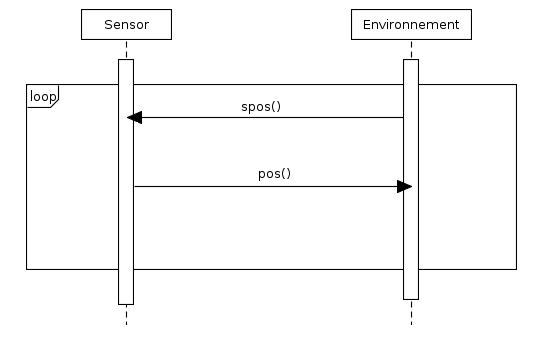
\includegraphics[scale=0.25]{./images/diagSeqExemple.png}

    \begin{block}{Simplifications}
        \begin{itemize}
            \item Red�finition de noms
            \item Abandon synchronisation des messages
            \item Garde les �l�ments utiles
            \item Ajoute de nouveaux �l�ments

        \end{itemize}

    \end{block}

\end{frame}

\begin{frame}{M�ta mod�le du diagramme de s�quences SysML}
    \centering
    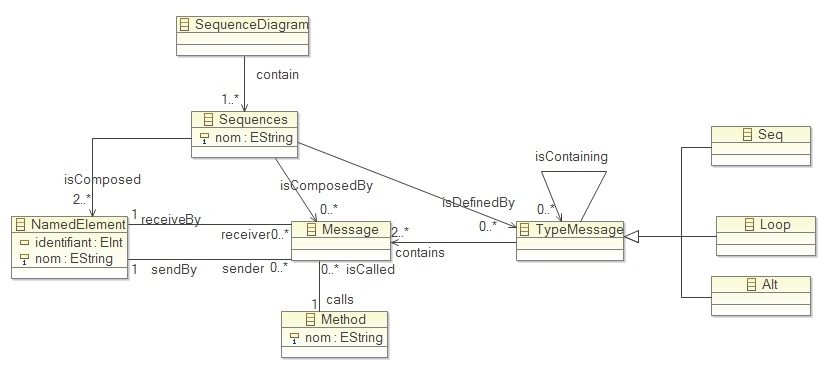
\includegraphics[scale=0.5]{./images/MMDiagSeq.jpg}

\end{frame}

\begin{frame}{M�ta mod�le du langage Ticc}
    \centering
    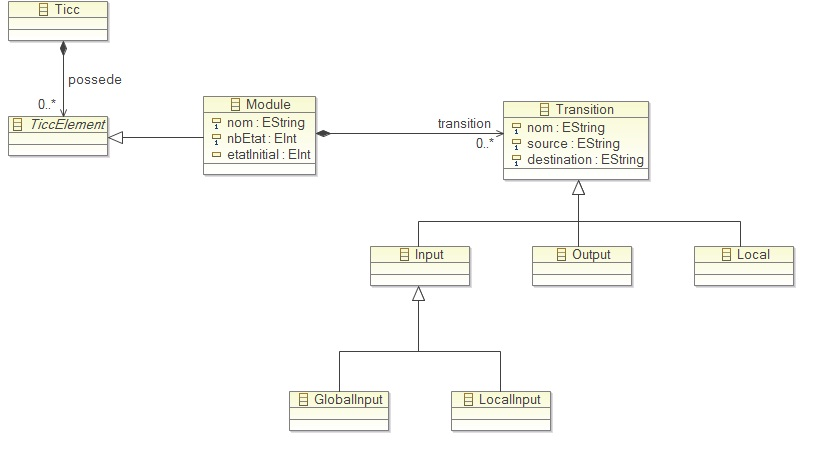
\includegraphics[scale=0.5]{./images/MMTicc.jpg}

\end{frame}

%

\subsection{Exemple fichier conforme au diagramme de s�quence}
\begin{frame}{Fichier d'entr�e}
    \begin{block}{Explication}
        \begin{itemize}
            \item Fichier de type XMI (XML Metadata Interchange)
            \item Conforme au m�ta mod�le du diagramme de s�quence
            \item Contient deux s�quences
            \item Une s�quence re�oit/envoi des messages de/� l'ext�rieur 
            vers un composant appel� \textit{Environnement} 

        \end{itemize}

    \end{block}

\end{frame}

%

\subsection{R�gles ATL}
\begin{frame}{But des r�gles ATL}
    \centering
    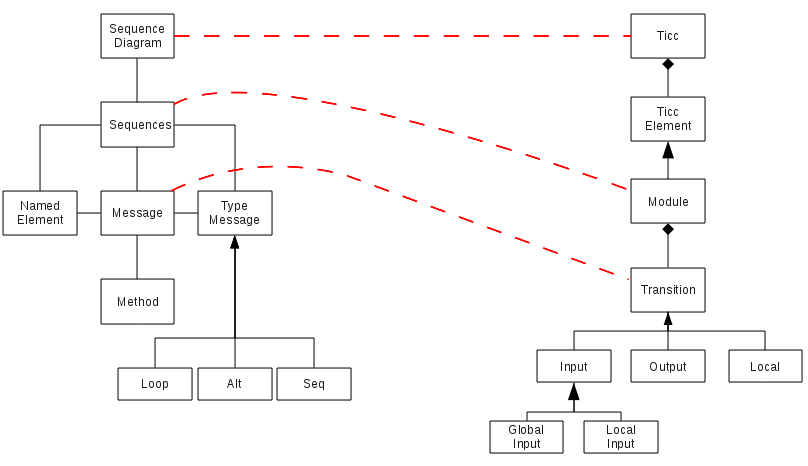
\includegraphics[scale=0.5]{./images/figureSimilitudeSeqTicc.png}

\end{frame}

%

\subsection{Parseur XML}
\begin{frame}{Parseur XML}
    \centering
    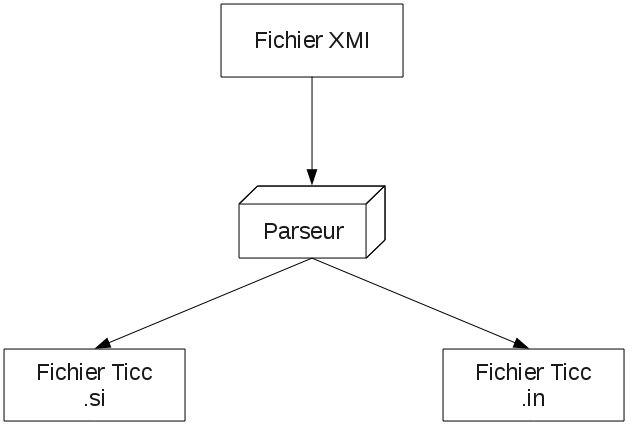
\includegraphics[scale=0.3]{./images/figureParseur.jpg}

    \begin{block}{Explications}
        \begin{itemize}
            \item Fichier de sortie XMI conforme Ticc 
            \item Traitement avec JDom
            \item G�n�ration fichier .si contenant les modules
            \item G�n�ration fichier .in ex�cutable OCaml

        \end{itemize}

    \end{block}

\end{frame}

%

\subsection{Traitement Ticc}


